\documentclass{beamer}
\usepackage{graphicx}
\usepackage{amssymb}
\usepackage{fontspec, xltxtra,xunicode}
\usepackage[UTF8,noindent]{ctex}
\usepackage{bbm}
\usepackage{color}
\usepackage[ruled,vlined]{algorithm2e}
\usepackage{mathspec}
\mode<presentation> {
\usetheme{Madrid}
}
\usefonttheme{professionalfonts}
\usepackage{times}
\usepackage{graphicx} % Allows including images
\usepackage{booktabs} % Allows the use of \toprule, \midrule and \bottomrule in tables
\usepackage{subfigure}
\usepackage[backend=bibtex,sorting=none]{biblatex}
\usepackage{tikz}
\setbeamerfont{section in toc}{shape=\itshape,family=\rmfamily}
\setbeamerfont{footline}{shape=\itshape,family=\rmfamily}
\setbeamerfont{title}{shape=\itshape,family=\rmfamily}
\setbeamerfont{author}{shape=\itshape,family=\rmfamily}
\setbeamerfont{institute}{shape=\itshape,family=\rmfamily}
\setbeamerfont{date}{shape=\itshape,family=\rmfamily}
\setbeamerfont{frametitle}{shape=\itshape,family=\rmfamily}
\setbeamerfont{block title}{shape=\itshape,family=\rmfamily}
\setbeamerfont{block body}{shape=\itshape,family=\rmfamily}
\setbeamerfont{footnote}{shape=\itshape,family=\rmfamily}

\usebackgroundtemplate{
    \begin{tikzpicture}
    \useasboundingbox (0,0) rectangle (\paperwidth,\paperheight);
    \node[at=(current page.center), inner sep=0pt, opacity=0.8] {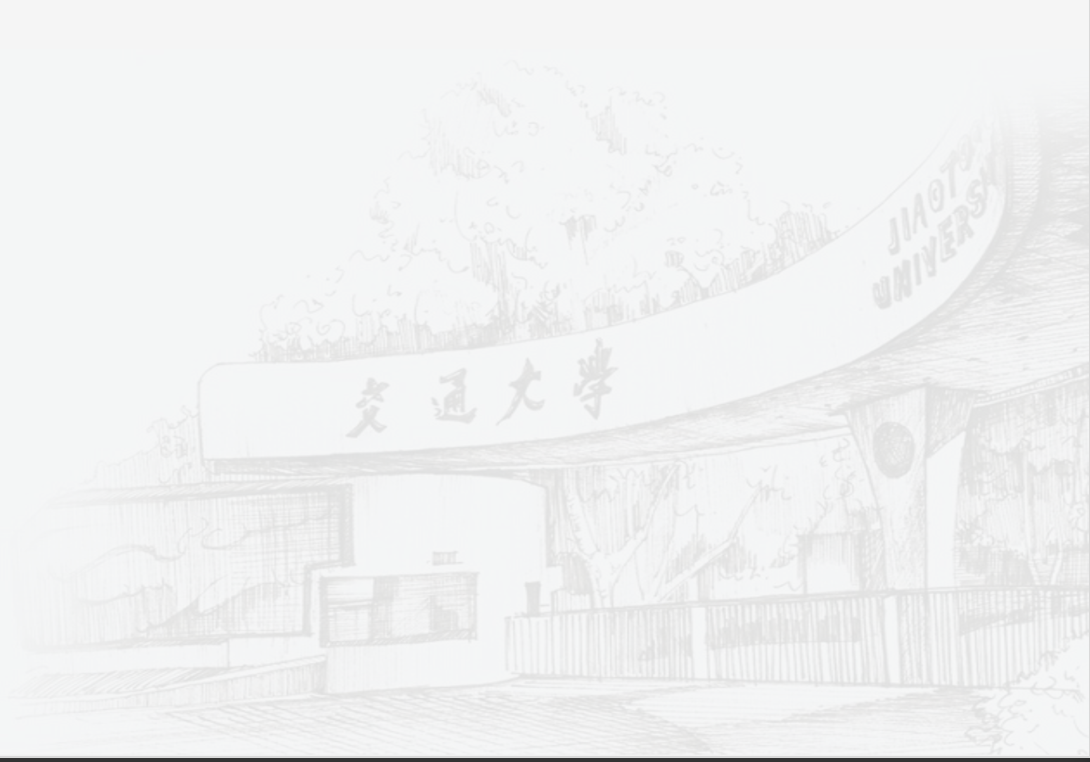
\includegraphics[width=\paperwidth,height=\paperheight]{../../pics/xjtu_draw.png}};
    \end{tikzpicture}
}
\definecolor{darkblue}{RGB}{10,80,152}
\definecolor{deepblue}{RGB}{181,203,223}
\definecolor{plainblue}{RGB}{228,235,245}
\setbeamercolor{block body}{bg=plainblue}
\setbeamercolor{block title}{fg=darkblue,bg=deepblue}
\linespread{1.2}
\setbeamertemplate{frametitle}
{
    \vspace{-14pt} % 减少顶部间距
    \nointerlineskip % 删除额外的行间距
    \begin{beamercolorbox}[wd=\paperwidth,ht=2.2em,dp=0.5em,leftskip=8pt,rightskip=0pt]{frametitle} % 调整高度参数
    \usebeamerfont{frametitle}\strut\insertframetitle\strut
    \end{beamercolorbox}
    \vspace{-6pt} % 减少底部间距
}

%----------------------------------------------------------------------------------------
%	TITLE PAGE
%----------------------------------------------------------------------------------------
% \footnote[frame]{\fullcite{wangneural}}
\title[Structure Learning with SDE]{\huge 基于随机微分方程的结构学习\footnote[frame]{\fullcite{wangneural}}}
\subtitle{\large  \rightline{时间序列因果学习的连续建模方法}} % The short title appears at the bottom of every slide, the full title is only on the title page

\author[王一丁]{王一丁} % Your name
\vspace{1em}
\date{2024年7月8日} % Date, can be changed to a custom date



\addbibresource{refs.bib} %BibTeX数据文件及位置
\setbeamerfont{footnote}{size=\tiny}

\begin{document}
\itshape
\rmfamily

\begin{frame}
\titlepage % Print the title page as the first slide

\end{frame}


\AtBeginSection[]
{
  \begin{frame}
    \frametitle{目录}
    \tableofcontents[currentsection]
  \end{frame}
}
\AtBeginSubsubsection[]
{
  \begin{frame}
    \frametitle{目录}
    \tableofcontents[currentsection,currentsubsection,currentsubsubsection]
  \end{frame}
}
%----------------------------------------------------------------------------------------
%	PRESENTATION SLIDES
%----------------------------------------------------------------------------------------

%------------------------------------------------
\section{绪论} % Sections can be created in order to organize your presentation into discrete blocks, all sections and subsections are automatically printed in the table of contents as an overview of the talk
%------------------------------------------------


\begin{frame}
\frametitle{问题引入及分析}
时间序列数据在现实世界中无处不在,通常由在不同时间间隔记录的一系列数据点组成。理解与时间过程相关的变量之间的底层因果结构对于许多现实世界的应用至关重要。
\\~\\
\begin{block}{现有离散时间结构学习的不足之处}
\begin{itemize}
    \item 当真正的底层过程连续,可能推断出不正确的因果关系。
    \item 难以处理不规则的采样间隔。
\end{itemize}
\end{block}
\vspace{1em}
本文引入了一种新的框架,采用随机微分方程(SDEs)作为\textcolor{red}{连续的隐过程}学习时间序列中的因果结构。
\end{frame}

\begin{frame}
\frametitle{文章贡献}
\begin{block}{文章贡献}
\begin{itemize}
    \item 与之前使用常微分方程的方法相比,该模型能够从\textcolor{red}{多模态\footnote[frame]{该模型同时学习多个时间序列共同的因果关系,可能对多模态学习有帮助,但是实验部分并未使用多模态数据进行证实。}}和\textcolor{red}{非高斯分布}的时序数据中准确地学习潜在的因果关系。
    \item 证明了当SDEs直接用于观测过程的建模时,所得到的SDEs在全局Lipschitz和对角扩散假设下是\textcolor{red}{结构可识别}的。
    \item 对合成的有真实背景的数据集进行了\textcolor{red}{广泛的实验},表明SCOTCH可以改进现有的结构学习方法,包括当处理不规则抽样数据\footnote[frame]{在实验部分,作者随机丢弃时间序列中的数据来模拟不规则抽样。}时。
\end{itemize}
\end{block}
\end{frame}

\section{预备知识}
\begin{frame}
\frametitle{贝叶斯结构学习}

\textcolor{red}{目的:从观测数据中学习表示结点之间的有向关系图(因果图)}。

给定时间序列数据 $\{\boldsymbol X_{t_i}\}_{i=1}^{I}$ ,包含 $I$ 个时间点。假设有 $N$ 个独立同分布的数据,给定图 $\boldsymbol G\in\{0,1\}^{D\times D}$,定义图与数据的联合分布:
\begin{equation}\scalebox{0.9}{$
p(\boldsymbol{G},\boldsymbol{X}^{(1)},\cdots,\boldsymbol{X}^{(N)})=p(\boldsymbol{G})\prod_{n=1}^{N}p(\boldsymbol{X}^{(n)}|\boldsymbol{G})$}
\end{equation}

其中 $p(\boldsymbol{G})$ 是图的先验分布,$p(\boldsymbol{X}^{(n)}|\boldsymbol{G})$ 是似然项。

目的是学习后验分布 $p(\boldsymbol G|\boldsymbol X^{(1)},\cdots, \boldsymbol X^{(N)})$ :
\begin{equation}\scalebox{0.9}{$
\begin{aligned}
     p(\boldsymbol{G}|\boldsymbol X^{(1)},\cdots, \boldsymbol X^{(N)})&=\dfrac{p(\boldsymbol{G},\boldsymbol{X}^{(1)},\cdots,\boldsymbol{X}^{(N)})}{p(\boldsymbol{X}^{(1)},\cdots,\boldsymbol{X}^{(N)})}\\
    &=\dfrac{p(\boldsymbol{G})\prod_{n=1}^{N}p(\boldsymbol{X}^{(n)}|\boldsymbol{G})}{\sum_{\boldsymbol{G}}p(\boldsymbol{G})\prod_{n=1}^{N}p(\boldsymbol{X}^{(n)}|\boldsymbol{G})}
\end{aligned}$}
\end{equation}
    % p(\boldsymbol{G}|\boldsymbol X^{(1)},\cdots, \boldsymbol X^{(N)})&=\dfrac{p(\boldsymbol{G},\boldsymbol{X}^{(1)},\cdots,\boldsymbol{X}^{(N)})}{p(\boldsymbol{X}^{(1)},\cdots,\boldsymbol{X}^{(N)})}\\
  %  &=\dfrac{p(\boldsymbol{G})\prod_{n=1}^{N}p(\boldsymbol{X}^{(n)}|\boldsymbol{G})}{\sum_\boldsymbol{G} p(\boldsymbol{G})\prod_{n=1}^{N}p(\boldsymbol{X}^{(n)}|\boldsymbol{G})}
但是由于图 $\boldsymbol{G}$ 所在的空间维度很高,难以准确计算上述后验分布,可以使用变分推断与采样来学习。
\end{frame}

\begin{frame}
\frametitle{结构方程模型 (SEM)}
给定时间序列数据 $\{\boldsymbol X^{(n)}\}_{n=1}^{N}$ 和图 $\boldsymbol G\in\{0,1\}^{D\times D}$ ,可以使用 SEM 描述变量间的结构关系:
\begin{equation}
    \boldsymbol X_{t,d}=f_{t,d}(Pa_{\boldsymbol{G}}^d(<t),\epsilon_{t,d})
\end{equation}
$Pa_{\boldsymbol{G}}^d(<t)$ 表示父节点在之前时刻的数据, $\epsilon_{t,d}$ 表示相互独立的噪声。
\\~\\
该模型需要\textcolor{red}{离散的时间步长\footnote[frame]{这里的离散主要说的是数据生成的因果结构是离散的,这导致了如果数据的因果频率与采样频率不一致的话,将很难发现数据中的因果关系。将底层因果结构建模为连续系统的话将没有这种问题,虽然最终经过采样还是会落到离散点,但是底层的连续性保证了采样点足够多便可以逼近真实过程(有点像采样定理)。}},这些时间步长通常被假定为遵循规则的采样间隔。现有模型大多遵循此框架。
\end{frame}

\begin{frame}
\frametitle{伊藤扩散过程 (It\^o diffusion)}
假设 $\boldsymbol X_t$ 是非时变\footnote[frame]{非时变是指 $f(\boldsymbol X_t),g(\boldsymbol X_t)$ 不随时间 $t$ 变化。作者在文中提到,采用非时变有助于证明结构可识别性,并在展望部分提出可能需要引入新的理论和方法来应对“动态因果”。} (time-homogenous) 的伊藤过程,则
\begin{equation}
    d\boldsymbol X_t=f(\boldsymbol X_t)dt+g(\boldsymbol X_t)d\boldsymbol W_t
\end{equation}
其中 $f:\mathbb{R}^D\to\mathbb{R}^D,g:\mathbb{R}^D\to\mathbb{R}^{D\times D}$ 分别是非时变的漂移项和扩散项。$\boldsymbol W_t$ 是测度 $P$ 下的布朗运动。

若全局Lipschitz条件满足,则 (3) 式有唯一强解\footnote[frame]{\fullcite{oksendal2003stochastic} (Thm 5.2.1)}:
\begin{equation}\scalebox{0.9}{$
    \boldsymbol X_t=\lim\limits_{n\to\infty}\boldsymbol Y_t^{(n+1)}=\lim\limits_{n\to\infty}\left(\boldsymbol X_0+\int_0^tf(\boldsymbol Y_s^{(n)})ds+\int_0^tg(\boldsymbol Y_s^{(n)})dB_s\right)$}
\end{equation}
其中 $\boldsymbol Y_{t}^{(0)}=\boldsymbol X_{0}$,$\boldsymbol Y_{t}^{(k)}=\boldsymbol Y_{t}^{(k)}(\omega)$ 

但是对于大多数拥有非线性漂移和扩散函数的伊藤扩散过程,解析解 $\boldsymbol X_t$ 是难以得到的,因此需要使用\textcolor{red}{离散化}的方式解决。
\end{frame}


\begin{frame}
\frametitle{Euler SEM}
固定步长 $\Delta$ ,使用 Euler 离散化可得轨迹:
\begin{equation}
    \boldsymbol X_{t+1}^\Delta=\boldsymbol X_t^\Delta+f(\boldsymbol X_t^\Delta)\Delta+g(\boldsymbol X_t^\Delta)\eta_t
\end{equation}
在图 $\boldsymbol G$ 中,定义结点 $i$ 不是结点 $j$ 在时刻 $t$ 的因,若对于任意 $k$ ,$\dfrac{\partial f_{j}(X_{t}^{\Delta})}{\partial X_{t,i}^{\Delta}}=0$,且 $\dfrac{\partial g_{j,k}(X_{t}^{\Delta})}{\partial X_{t,i}^{\Delta}}=0$ 。
\\~\\
如果假设 $g$ 输出对角矩阵,则上述 Euler 离散化可以导出时序SEM\footnote[frame]{此时漂移项部分 $g(\boldsymbol X_t^\Delta)\eta_t$ 和 $t$ 时刻数据 $\boldsymbol X_t^\Delta$ 的维度一致,因此可看作是 SEM 中噪声 $\boldsymbol{\epsilon}_{t}$的变体。},被称为 Euler SEM。
\end{frame}
\section{SCOTCH}
\begin{frame}
\frametitle{模型引入}
考虑一个动力系统,\textcolor{red}{既拥有内在的随机性,也被外界的噪声干扰}。例如,在医疗保健中,患者的病情将随机发展,而不是确定性。此外,患者状况的测量也会受到设备精度的影响,其中噪声与内在随机性无关。
\\~\\
因此引入潜在随机微分方程模型:
\begin{equation}
\begin{aligned}
d\boldsymbol Z_t=f_\theta(\boldsymbol Z_t)dt+g_\theta(\boldsymbol Z_t)d\boldsymbol W_t\quad&\text{(隐过程)}\\
\boldsymbol X_t=\boldsymbol Z_t+\boldsymbol \epsilon_t\quad&\text{(带噪观测过程)}
\end{aligned}
\end{equation}
其中 $\boldsymbol Z_t$ 是系统内部状态的潜在变量,$\boldsymbol X_t$ 是具有相同维度的观测数据,$\boldsymbol W_t$ 是Wiener过程(物理意义为布朗运动)。
\end{frame}

\begin{frame}
\frametitle{模型假设}
\begin{block}{假设1:全局Lipschitz}
    上式中的漂移和扩散函数满足全局Lipschitz约束。也就是说
\vspace{-10pt}
\begin{equation}
    |\boldsymbol f_\theta(\boldsymbol x)-\boldsymbol f_\theta(\boldsymbol y)|+|\boldsymbol g_\theta(\boldsymbol x)-\boldsymbol g_\theta(\boldsymbol y)|\leq C|\boldsymbol x-\boldsymbol y|
\end{equation}
\end{block}
假设1是大多数 SDE 文献要求的标准假设,以确保存在强解。
\\~\\
\begin{block}{假设2:对角扩散}
    扩散函数输出一个非零对角线矩阵。也就是说,它可以简化为向量值函数 $\boldsymbol g_\theta(\boldsymbol X_t):\mathbb R^D\to\mathbb R^D$ 
\end{block}
假设2帮助证明了结构可识别性。
\end{frame}

\begin{frame}
\frametitle{过程先验}
由于潜过程在看到任何观测值之前就诱导了潜轨迹的分布,因此也将其称为先验过程。本文使用类似\textcolor{red}{掩码}的方法,将图 $\boldsymbol G$ 与隐空间表征做内积来学习因果。并将\textcolor{red}{神经网络}嵌入在漂移函数 $\boldsymbol f_\theta (\cdot,\boldsymbol G)$ 与扩散函数 $\boldsymbol g_\theta (\cdot,\boldsymbol G)$ 的表示中:
\begin{equation}
    \boldsymbol f_{\theta,d}(\boldsymbol Z_t, G)=\zeta\left(\sum_{i=1}^DG_{i,d}l(Z_{t,i},\boldsymbol e_i),\boldsymbol e_d\right)
\end{equation}
其中 $\zeta,l$ 是神经网络,$\boldsymbol e_i$ 是共享的可训练的结点嵌入。
\\~\\
综上,过程先验可表示为:
\begin{equation}
    d\boldsymbol Z_t=\boldsymbol f_\theta(\boldsymbol Z_t,\boldsymbol G)dt+\boldsymbol g_\theta(\boldsymbol Z_t,\boldsymbol G)d\boldsymbol W_t\quad\text{(先验过程)}
\end{equation}
该先验过程中的参数可随着训练过程迭代。
\end{frame}
\begin{frame}
\frametitle{图先验与似然}
\begin{block}{图先验}
    \begin{equation}
        p(\boldsymbol G)\propto\exp(-\lambda_s\|\boldsymbol G\|_F^2)
    \end{equation}
    其中 $\lambda_s$ 是稀疏系数。
\end{block}
\begin{block}{似然}
    \begin{equation}
        p(\{\boldsymbol X_{t_{i}}\}_{i=1}^{I}|\{\boldsymbol Z_{t_{i}}\}_{i=1}^{I},\boldsymbol G)=\prod_{i=1}^{I}\prod_{d=1}^{D}p_{\epsilon_{d}}(X_{t_{i},d}-Z_{t_{i},d})
    \end{equation}
该似然表示了噪声的分布。
\end{block}
\end{frame}
\begin{frame}
\frametitle{变分推断}
假设 $\{\boldsymbol X^{(n)}\}_{n=1}^{N}$ 是系统中的观测数据,目标是学习数据中的图结构 $\boldsymbol p(\boldsymbol G|\{\boldsymbol X^{(n)}\}_{n=1}^{N})$ \footnote[frame]{文章假设所有数据来自同一个因果系统生成,fMRI分析可能不太适用,因为每个个体可能存在差异。},这是无法直接学习的,因此采用变分推断。
\vspace{10pt}

变分近似:$q_\phi(\boldsymbol G)\approx p(\boldsymbol G|\boldsymbol X^{(1)},\cdots,\boldsymbol X^{(N)})$ 。

变分下界计算:
\vspace{-5pt}
\begin{equation}\scalebox{0.85}{$
    \log p(\boldsymbol{X}^{(1)},\cdots,\boldsymbol{X}^{(N)})\geq\mathbb{E}_{q_\phi(\boldsymbol{G})}\left[\sum_{n=1}^N\log p_\theta(\boldsymbol{X}^{(n)}|\boldsymbol{G})\right]-D_{\text{KL}}(q_\phi(\boldsymbol{G})\|p(\boldsymbol{G}))$}\end{equation}
\vspace{-10pt}

由于存在隐空间 $\boldsymbol Z^{(n)}$ ,故 $p_\theta(\boldsymbol{X}^{(n)}|\boldsymbol G)$ 无法直接计算,因此首先使用变分框架估计后验分布 $p(\boldsymbol Z^{(n)}|\boldsymbol G,\boldsymbol X^{(n)})$,变分后验 $q_\psi(\tilde{\boldsymbol Z}^{(n)}|\boldsymbol G,\boldsymbol X^{(n)})$ 被定义为如下系统的解:
\vspace{-5pt}
\begin{equation}\scalebox{0.85}{$
\begin{aligned}
\tilde{\boldsymbol Z}_{t,0}^{(n)}\sim\mathcal{N}(\mu_{\psi}(\boldsymbol G,\boldsymbol X^{(n)}),\Sigma_{\psi}(\boldsymbol G,\boldsymbol X^{(n)}))\quad&\text{(后验初始状态)}\\d\tilde{\boldsymbol Z}_{t}^{(n)}=h_{\psi}(\tilde{\boldsymbol Z}_{t}^{(n)},t;\boldsymbol G,\boldsymbol X^{(n)})dt+g_{\boldsymbol G}(\tilde{\boldsymbol Z}_{t}^{(n)})d\boldsymbol W_{t}\quad&\text{(后验过程)}
\end{aligned}$}
\end{equation}
\end{frame}
\begin{frame}
\frametitle{变分推断}
\begin{equation*}
\begin{aligned}
\tilde{\boldsymbol Z}_{t,0}^{(n)}\sim\mathcal{N}(\mu_{\psi}(\boldsymbol G,\boldsymbol X^{(n)}),\Sigma_{\psi}(\boldsymbol G,\boldsymbol X^{(n)}))\quad&\text{(后验初始状态)}\\d\tilde{\boldsymbol Z}_{t}^{(n)}=h_{\psi}(\tilde{\boldsymbol Z}_{t}^{(n)},t;\boldsymbol G,\boldsymbol X^{(n)})dt+g_{\boldsymbol G}(\tilde{\boldsymbol Z}_{t}^{(n)})d\boldsymbol W_{t}\quad&\text{(后验过程)}
\end{aligned}
\end{equation*}
初始状态由\textcolor{red}{神经网络}学习到的均值和方差表示。后验扩散函数与先验相同(由于扩散函数类似噪声,与数据无关)。
\begin{block}{后验漂移函数与先验不同的两点理由}
    \begin{itemize}
        \item 后验漂移函数取决于时间,即使因果是非时变的。不同时间下即使是相同的数据,可能有不同的运动趋势。
        \item 不受限于先验掩码结构,从而可以表示更加复杂的系统。
    \end{itemize}
\end{block}
\end{frame}
\begin{frame}
\frametitle{变分推断}
接着,根据之前文献\footnote[frame]{\fullcite{li2020scalable}}的理论,$\log p(\boldsymbol{X}^{(n)}|\boldsymbol{G})$ 有下界:
\begin{equation}\scalebox{0.78}{$
    \log p(\boldsymbol{X}^{(n)}|\boldsymbol{G})\geq\mathbb{E}_{q_\psi}\left[\sum_{i=1}^I\log p(\boldsymbol{X}_{t_i}^{(n)}|\tilde{\boldsymbol{Z}}_{t_i}^{(n)},\boldsymbol{G})-\int_0^T\|\boldsymbol{u}^{(n)}(\tilde{\boldsymbol{Z}}_t^{(n)})\|^2dt\right]$}
\end{equation}
其中:
\begin{equation}\scalebox{0.78}{$
    u^{(n)}(\tilde{\boldsymbol Z}_t^{(n)})=g_G(\tilde{\boldsymbol Z}_t^{(n)})^{-1}(h_\psi(\tilde{\boldsymbol Z}_t^{(n)},t;\boldsymbol G,\boldsymbol X^{(n)})-f_G(\tilde{\boldsymbol Z}_t^{(n)}))$}
\end{equation}
因此总体证据下界为:
\begin{equation}
    \scalebox{0.78}{$\mathbb{E}_{q_{\phi}}\left[\sum\limits_{n=1}^{N}\mathbb{E}_{q_{\psi}}\left[\sum\limits_{i=1}^{I}\log p(\boldsymbol X_{t_{i}}^{(n)}|\tilde{\boldsymbol Z}_{t_{i}}^{(n)},\boldsymbol G)-\int_{0}^{T}\|\boldsymbol u^{(n)}(\tilde{\boldsymbol Z}_{t}^{(n)})\|^{2}dt\right]\right]-D_{\mathrm{KL}}(q_{\phi}(\boldsymbol{G})\|p(\boldsymbol{G}))$}
\end{equation}
实际计算中使用 Monte-Carlo 方法近似上式中的期望。
\end{frame}

\begin{frame}
\frametitle{SCOTCH算法}
\begin{equation*}
    \scalebox{0.78}{$\mathbb{E}_{q_{\phi}}\left[\sum\limits_{n=1}^{N}\mathbb{E}_{q_{\psi}}\left[\sum\limits_{i=1}^{I}\log p(\boldsymbol X_{t_{i}}^{(n)}|\tilde{\boldsymbol Z}_{t_{i}}^{(n)},\boldsymbol G)-\int_{0}^{T}\|\boldsymbol u^{(n)}(\tilde{\boldsymbol Z}_{t}^{(n)})\|^{2}dt\right]\right]-D_{\mathrm{KL}}(q_{\phi}(\boldsymbol{G})\|p(\boldsymbol{G}))$}
\end{equation*}
\begin{figure}[htbp]
\centering  
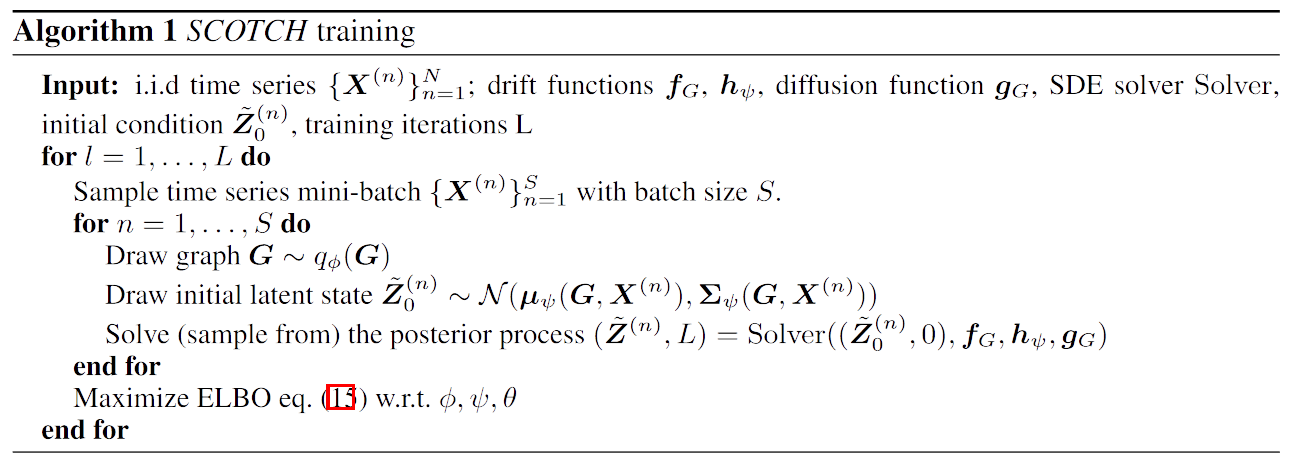
\includegraphics[width=\linewidth]{SCOTCH.png}
\caption{SCOTCH算法}
\end{figure}

\end{frame}

\section{理论分析}
\begin{frame}
\frametitle{结构可识别性定理}
假设观察过程是作为It\^o扩散给出的:
\begin{equation} d\boldsymbol{X}_t=f_G(\boldsymbol{X}_t)dt+g_G(\boldsymbol{X}_t)d\boldsymbol{W}_t
\end{equation}
则模型在结构上可识别的充分条件由下述定理提供:
\begin{block}{定理1:观测过程的结构可识别性}
    给定上述方程,设有另一过程 $\bar{\boldsymbol X}_{t}, \boldsymbol G\neq\bar{\boldsymbol G}, \bar{\boldsymbol f}_{\bar{\boldsymbol G}}, \bar{\boldsymbol g}_{\bar{\boldsymbol G}}, \bar{\boldsymbol W}_{t}$,则在共同的初始值与假设1,2下,解 $\boldsymbol X_t,\bar{\boldsymbol X_t}$ 有不同的分布。
\end{block}
\end{frame}

\begin{frame}
\frametitle{结构可识别性定理}
下述定理表明,在某些条件下,即使没有直接观察到 SDE 的解,即存在隐过程 $\boldsymbol Z$,结构可识别性也可以保持。
\begin{block}{定理2:潜在过程的结构可识别性}
考虑由隐过程公式定义的两组分布 $p,\bar p$ ,分别对应 $(\boldsymbol G,\boldsymbol Z,\boldsymbol X,\boldsymbol f_{\boldsymbol G},\boldsymbol g_{\boldsymbol G})$,$(\bar {\boldsymbol G},\bar {\boldsymbol Z},\bar {\boldsymbol X},\bar {\boldsymbol f}_{\bar {\boldsymbol G}},\bar {\boldsymbol g}_{\bar {\boldsymbol G}})$ ,其中 $\boldsymbol G\ne\bar {\boldsymbol G}$。令 $t_1,\cdots,t_I$ 是观测的时间序列,则在假设1,2下,有
\begin{itemize}
    \item 若对任意 $i$,有 $t_{i+1}-t_i=\Delta$ ,则欧拉离散化 $p^{\Delta}(\boldsymbol X_{t_{1}},\cdots,\boldsymbol X_{t_{1}})\neq\bar{p}^{\Delta}(\bar{\boldsymbol X}_{t_{1}},\cdots,\bar{\boldsymbol X}_{t_{1}})$
    \item 如果固定时间范围 $[0,T]$,则采样点数趋近无穷时 $p(\boldsymbol X_{t_{1}},\cdots,\boldsymbol X_{t_{1}})\neq\bar{p}(\bar{\boldsymbol X}_{t_{1}},\cdots,\bar{\boldsymbol X}_{t_{1}})$ 
\end{itemize}
\end{block}
\end{frame}

\begin{frame}
\frametitle{一致性定理}
在结构可识别性的基础上,可以证明变分公式的一致性。也就是说,在无限数据限制下,可以通过使用足够表达的后验过程和正确指定的模型最大化ELBO来恢复真值图。
\begin{block}{定理3:变分表述的一致性}
    若假设 1-2 满足潜在公式,则对于固定的观测时间范围 $[0,T]$,作为观测值数趋于无穷,当ELBO最大化时,$\boldsymbol q_\phi(\boldsymbol G)=\delta(\boldsymbol G^*)$,其中 $\boldsymbol G^∗$ 为真值图。
\end{block}
\end{frame}


\section{实验分析}


    
\section{总结与展望}
\begin{frame}
\frametitle{总结与展望}
\begin{itemize}
    \item 本文提供的连续时间因果发现框架解决了离散学习中遇到的采样频率与真实因果频率不一致等问题。
    \item 本文的结构可识别性证明框架奠定了连续时序因果发现的基础。
    \item 使用了广泛的可下载的数据集。
    \item 可以考虑将其拓展至动态因果。
\end{itemize}
\end{frame}

\begin{frame}
  \frametitle{参考文献}
  \printbibliography
\end{frame}

\begin{frame}
\Huge{\centerline{谢谢!}}
\end{frame}
%------------------------------------------------

%----------------------------------------------------------------------------------------

\end{document} 